\documentclass[tikz,border=3mm]{standalone}
\usepackage{tikz-feynman}
\begin{document}
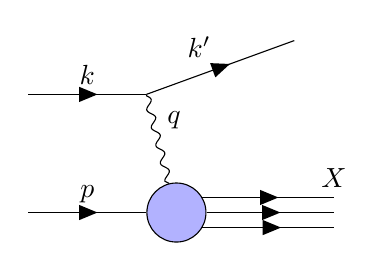
\begin{tikzpicture}
\begin{feynman}[every blob={/tikz/fill=blue!30,/tikz/inner sep=2pt}]
\vertex (li);
\vertex [below=1.5cm of li] (hi);
\vertex [right=of li] (a);
\path (a) ++ (20:2) node[vertex] (lf);
\vertex [below right=of a] (b);
\vertex [blob, right=of hi] (c) {};
\path (c) ++ (00:2) node[vertex] (hf2);
\path (c.-30-|hf2.center) node[vertex] (hf3);
\path (c.+30-|hf2.center) node[vertex, label=\(X\)] (hf1);

\diagram* {
    (li) -- [fermion, edge label=\(k\)] (a) -- [fermion, edge label=\(k'\)] (lf),
    (hi) -- [fermion, edge label=\(p\)] (c),
    (a) -- [photon, edge label=\(q\)] (c),
    (c.+30) -- [fermion] (hf1),
    (c) -- [fermion] (hf2),
    (c.-30) -- [with arrow=0.52] (hf3)
};
\end{feynman}
\end{tikzpicture}
\end{document}
